% -------------------------------------------------------------------------------------
% Plantilla para escribir una tesis de la Universidad Nacional de Colombia en LaTeX
% *************************************************************************************
% -------------------------------------------------------------------------------------
\PassOptionsToPackage{spanish,english}{babel}
\documentclass[]{thesisUnal}
% -------------------------------------------------------------------------------------
% Espacio reservado para la carga de los paquetes por parte del autor
% **** --------------------------------------------------------------------------------

\usepackage[spanish]{babel}
\usepackage{rotating}
\usepackage{inputenx}
\usepackage[T1]{fontenc}
\usepackage{amsmath}
\usepackage{amssymb}
%\usepackage[spanish,activeacute,es-tabla]{babel}
%\usepackage[utf8]{inputenc}
\usepackage{amsmath, amsthm, amsfonts}
\usepackage{graphicx} % LaTeX
\usepackage{float} % LaTeX
%\usepackage{natbib} % bibliograf�a
%\usepackage{enumitem}

% //// --------------------------------------------------------------------------------
% -------------------------------------------------------------------------------------
% Espacio reservado para colocar las definiciones especiales por parte del autor
% **** --------------------------------------------------------------------------------




%%%%%%%%%%%%%%%%%%%%%%%%%%%%%%%%%%%%%%%%%%%%%%%%%%%%%%%%%%%%%%%%%%%%%%%%%%%%%%%%%%%%%%%
% \includeonly{cap1,cap2}
%%%%%%%%%%%%%%%%%%%%%%%%%%%%%%%%%%%%%%%%%%%%%%%%%%%%%%%%%%%%%%%%%%%%%%%%%%%%%%%%%%%%%%%
% //// --------------------------------------------------------------------------------
% -------------------------------------------------------------------------------------
% * CUERPO DEL DOCUMENTO
% **** --------------------------------------------------------------------------------
% -------------------------------------------------------------------------------------
\begin{document}

\logouniversity[45mm]{imagesThesis/logo_university_nacho}

\infothesis[
    author = {Sergio David Solano Bejarano},
    degreeauthor = {Ingeniero Industrial},
    %code = {000000},
    advisor = {B. Piedad Urdinola Contreras, Ph.D.},
    degreeadvisor = {Doctor en Demograf�a},
    %coadvisor = {Jonatan Gom�z Perdomo, Ph.D.},
    %degreecoadvisor = {Doctora en Demograf�a},
    title = {Proyecci�n de poblaciones carcelarias en Colombia},
    titledegree = {Disertaci�n presentada para optar al t�tulo de},
    degree = {Master en Ciencias - Estad�stica},
    researchline = {Demograf�a},
    %researchgroup = {\LaTeX: para el fomento del uso de \LaTeX\ en la investigaci�n},
    university = {Universidad Nacional de Colombia},
    faculty = {Facultad de Ciencias},
    department = {Departamento de Estad�stica},
    city = {Bogot�, D.C.},
    date = {Abril de 2017},
]

\abstractthesis[
    titlespanish = {Proyecci�n de poblaciones carcelarias en Colombia},
    titleenglish = {Prison populations projections for Colombia},
    abstractspanish = {Se presentan proyecciones de poblaci�n carcelaria cuando no se conocen las tasas de ingreso al sistema carcelario, el tiempo de juicio, ni la duraci�n de la pena. Para estimar estas variables no observadas se utilizan modelos estado espacio multivariados, tomando como base la poblaci�n sindicada y condenada mensual},
    abstractenglish = {Not there yet!},
    keywordspanish = {Poblaciones carcelarias, series de tiempo, procesos SARIMA, Modelos Estado Espacio},
    keywordenglish = {Prison populations, time series, SARIMA processes, State Space Models},
]

\acceptationnote[
    note = {Aprobado},
    mention = {Meritoria o Laureada},
    jury = {Jurado uno},
    jury = {Jurado dos},
    %jury = {Michel Goossens},
    advisor = {B. Piedad Urdinola},
    %coadvisor = {Jonatan Gom�z},
    date = {Bogot�, D.C., Abril 19 de 2017}
]

\frontmatter
    \dedicatory{dedicatoria}
    \acknowledgement{agradecimientos}
    \tableofcontents
    \listoftables
    \listoffigures
    \introduction{introduccion}
\mainmatter
	\chapter{Antecedentes te�ricos}

En 2016 Colombia ocupa el puesto catorce entre doscientos cincuenta y un paises por el tama�o de su poblaci�n carcelaria (120 914 hbts.) y el cincuenta y uno seg�n la tasa de encarcelamiento (240 por cada 100.000 hbts). Tasa que pas� de 51,5 en  el a�o 2000 a 240 por cada 100.000 hbts en 2016. Con una ocupaci�n del 154\% de las plazas disponibles, resulta relevante contar con proyecciones de la poblaci�n carcelaria en el corto, mediano y largo plazo. \cite{InstitueforCriminalPolicyResearch2016}

\section{Proyecciones de poblaci�n}

"Una estimaci�n poblacional consiste en determinar el tama�o o las caracter�sticas de una poblaci�n, para el momento actual o para uno anterior, en ausencia de informaci�n. Cuando se realizan un conjunto de supuestos sobre el comportamiento de los vitales hacia el futuro, hablamos de proyecci�n, y cuando se escoge un escenario como el m�s probable, hablamos de pron�stico"\cite {Swanson2012}.

Para incluir la incertidumbre en las proyecciones de poblaci�n Lee enumera los siguientes m�todos \cite {Lee1994}: 
\begin{itemize}
	\item El enfoque de escenarios alto, medio y bajo: Asume comportamientos fijos para la fertilidad, la mortalidad y las migraciones durante el periodo de proyecci�n, basado en algunos supuestos \cite {Lee1994}.
	\item An�lisis estoc�sticos
	\begin{itemize}
		\item An�lisis ex-post: consiste en evaluar el error de pron�stico en proyecciones anteriores y aplicarlo a las nuevas proyecciones \cite {Lee1994}.
		\item Simulaci�n estoc�stica: Permite hacer proyecciones de poblaci�n, al asignar una distribuci�n de probabilidad a las tasas vitales (mortalidad, natalidad, migraciones) \cite {Lee1994}.
		\item Modelos estoc�sticos de la tasa de crecimiento: Consiste en estimar la tasa de crecimiento del total de la poblaci�n; aunque permite estimar intervalos de confianza, no permite separar la proyecci�n de las tasas vitales, ni de las franjas etarias \cite {Lee1994}.
		\item Matrices de Leslie con modelos estimados para las tasas vitales:  Al usar matrices de Leslie se estima la poblaci�n por rangos etarios para un instante i, y se calcula la poblaci�n en el instante i + 1 aplicando la natalidad y la mortalidad proyectadas para el periodo i. Puesto que las series de poblaci�n carcelaria no se publican separadas por edad, no se abordar� esta t�cnica.
	\end{itemize}
\end{itemize}

\subsection{Proyecci�n de poblaciones peque�as}

La proyecci�n de �reas peque�as es entendida como la proyecci�n a un nivel geogr�fico menor al nacional. Estas proyecciones pueden incluir, departamentos, ciudades o poblaciones especiales \cite {Swanson2012}.
"Una poblaci�n especial es un grupo poblacional que se encuentra restringido a un �rea por una medida administrativa o legislativa. Dentro de los grupos usualmente considerados se encuentran las prisiones, universidades, hospitales e instituciones militares".
Este tipo de poblaci�n puede tener una estructura etaria y de sexo,  y unos vitales diferentes al resto de la poblaci�n; adem�s no suelen envejecer en el mismo lugar, lo que permite mantener una estructura etaria que no var�a a trav�s del tiempo. \cite {Swanson2012}.

\subsection{Aplicaciones nacionales e internacionales}

Las proyecciones de poblaciones carcelarias oficiales analizadas corresponden, en buena parte, a los m�todos expuestos en los cap�tulos anteriores:  Proyecciones por escenarios, proyecci�n de la tasa de crecimiento, modelos ARIMA para las tasas de ingreso y salida.

En Colombia (CONPES 3828) se proyect� la poblaci�n carcelaria usando la tasa media de crecimiento anual (1993-2014) \cite {DepartamentoNacionaldePlaneacion2015}. Esta proyecci�n no tiene en cuenta la incertidumbre asociada con las variaciones aleatorias en las tasas, ni las asociadas a cambios estructurales.  

El Reino Unido hasta 2015 realizaba una proyecci�n por escenarios (alto, medio y bajo), a�o en el cual cambi� a un modelo de proyecci�n de la media y su incertidumbre. La incertidumbre se incluy� a trav�s de un an�lisis ex-post, de la  desviaci�n de la proyecci�n en a�os anteriores \cite {Justice2014}.

El departamento de Justicia de los Estados Unidos realiz� estimaciones de la poblaci�n carcelaria por estado para el periodo 2013-2014. Las estimaciones parten del censo de prisiones 1993-2014. Estas proyecciones se puede enmarcar dentro de las proyecciones de �reas peque�as \cite {Minton2015}.

El bureau de estad�sticas e investigaci�n del crimen en Australia proyecta las tasas de arresto y sentencia usando modelos ARIMA;  a partir de estas tasas proyecta la poblaci�n carcelaria. Estas proyecciones incluyen un periodo de validaci�n de tres a�os. Los resultados mostraban que la serie real se encuentra dentro de los intervalos de confianza de la proyecci�n, cercano a la proyecci�n de la media \cite{Wan1}.

Blummstein desarrolla un m�todo de proyecci�n basado en los componentes demogr�ficos, tasas espec�ficas de arresto por delito y reincidencias, a partir de estos datos proyecta el tama�o y la composici�n de las poblaciones \cite{Blumstein1980}.

Con los datos libres disponibles en Colombia no se podr�a utilizar el enfoque ARIMA ni el m�todo de Blummstein, pues las tasas de encarcelamiento y sentencia no se publican. La tesis busca proponer un m�todo de proyecci�n, para situaciones donde no se cuenta con el registro de los vitales o su equivalente en la poblaci�n analizada.

\section{Series de tiempo}

% SECCI�N EN PROCESO. 
% Una vez tenga una versi�n preliminar me encargar� de corregir y referenciar.

Una serie de tiempo es un conjunto de observaciones ${x_t}$ asociadas a un instante de tiempo t. Es usual referirse como series de tiempo, tanto a las realizaciones ${x_t}$ como a las variables aleatorias ${X_t}$ que las generan.\cite{Brockwell2011} 

En una regresi�n lineal cl�sica, una variable $Y$ es explicada o predicha en funci�n de una variable $X$. La diferencia entre el valor observado $y_i$ y el valor predicho se suponen provenientes de un proceso aleatorio con media cero. \cite{Commandeur2007}

\begin{center}
	$Y_i = \beta_{0} + \beta_{1} X_i + \epsilon_i$\\
\end{center}

Donde ${\epsilon_1, \epsilon_2, \epsilon_3}$ son independientes e id�nticamente distribuidas (i.i.d.). Es posible representar una serie de tiempo en esta forma, tomando como variable explicativa el tiempo. Sin embargo, el an�lisis de series de tiempo se ha desarrollado como un �rea particular de la estad�stica, pues es este supuesto no suele cumplirse, enfoc�ndose particularmente en variables aleatorias dependientes, que pueden ser representadas en la forma: 

\begin{center}
	$Y_i = \beta_{0} + \beta_{1} Y_1 + \beta_{2} Y_2 + ... + \beta_{i-1} Y_{i-1} + \ \epsilon_i$\\
\end{center}

Estacionaridad. 
Estacionaridad debil. 


C�mo se puede medir esto? con una funci�n de autocorrelaci�n, que mide la relaci�n entre los valores del proceso, seg�n su cercan�a. 

Time series is therefore primarily concerned with dependent random variables and the analysis and utilization of this dependence.) A simpler approach to forecastingXn+h is to look for the linear combi- nation, ? Xn+h = a0 +a1Xn +?+anX1 which minimizes the expected squared error E(Xn+h ? ? Xn+h) 2.Tis is a much simpler problem, the solution of which depends only on the expected values EXi and EXiXj, i, j = 1, 2, . . .Moreover if the joint distribution of (X1,X2, . . . ,Xk) is multivariate normal for every positive integer k then this best linear
forecast


Las series de tiempo tienen una aplicaci�n bastante limitada, pues requieren muchas (?) observaciones, espaciadas uniformemente. Cuando la correlaci�n se presenta en lags uniformente espaciados por ejemplo (12,24,36) se denomina una serie estacional. 

Para medir que tan bien ajusta el modelo analizamos el comportamiento del error de estimaci�n. Es usual suponer que el error tiene varianza constante (homocedasticidad), es  independiente e id�nticamente distribuido, usualmente con distribuci�n normal.

Es posible que el modelo tenga tendencia. Cuando la tendencia es lineal tomamos la diferencia al lag 1 (si queremos desestacionalizar, tomamos la diferencia al lag que nos sirve para desestacionalizar) y evaluamos  la autocorrelaci�n en esta nueva serie. (Expandir con libro del curso de Datacamp)

Cuando la varianza incrementa con el tiempo podemos asumir que el modelo crece de manera exponencial (un incremento porcentual fijo). Para manejar estas series de manera sencilla tomamos la logaritmo natural de la differencia entre pasos. (Expandir con Tsay) 


\subsection{Modelos ARIMA, SARIMA}

El an�lisis de las series tiempo de poblaciones carcelarias  de tiempo ARIMA y ARMAX se tomar� de \cite{Tsay2002}.


Los procesos ARMA son procesos aleatorios de la forma 

\begin{center}
	$Y_t = \gamma Y_{t-1} + \gamma_2 Y_{t-2} ...+ + \gamma_i Y_{t-i} + \epsilon + \theta_1\epsilon_{t-1} + \theta_2\epsilon_{t-2} ... \theta_j\epsilon_{t-j} $
\end{center}

A este modelo se le conoce como ARIMA(i,0,j).

Aunque el termino $\epsilon$ no tiene necesariamente una distribuci�n normal, por el resto de documento se asumir� una distribuci�n normal con media $\mu$ y varianza $\sigma�$, a menos que se especifique lo contrario. 

Los procesos ARIMA resultan al considerar una serie de la forma: 

\begin{center}
	$Y_t = \alpha +  Y_{t-1}$
\end{center}

Tal que el proceso $Y_t - Y_{t-1}$ es un proceso ARMA.

\subsection{Modelos Estado-Espacio}

Tomado de \cite{Lutkepohl2005} : 

En un modelo estado espacio una serie de tiempo (multiple) observada  $\ y_1, ... , y_t $\ depende de un estado $\ z_t $\ , posiblemente no observado, que se comporta siguiendo un proceso estoc�stico. La relaci�n entre $\ y_t $\ y $\ z_t $\ est� dada por la \textit{ecuaci�n de medida}: \cite{Lutkepohl2005}  

$\ y_t = H_t z_t + v_t$\

donde $\ H_t $\ es una matriz que puede o no depender del tiempo $\ t $\ y $\ v_t $\ es el error de observaci�n, que se asume usualmente como un proceso de ruido. El vector de estado es generado como:  

$\ z_t = B_{t-1} z_{t-1} + w_{t-1}$\

La matriz $\ B_t $\ es una matriz de coeficientes que puede depender de $\ t $\, y $\ w_t $\ es un proceso de ruido. \cite{Lutkepohl2005}

Es posible considerar los modelos estado-espacio una generalizaci�n de los modelo SARIMA y VARMA.
    \chapter{La poblaci�n carcelaria en Colombia 1991 - 2017}

\section{An�lisis exploratorio}

El INPEC publica mensualemente la serie poblaci�n carcelaria. Esta serie contiene la poblaci�n carcelaria desde 1991, separada por situaci�n jur�dica (condenados, sindicados) y genero.

La poblaci�n carcelaria total entre 1991 y 2017 se ha cuadruplicado, al pasar de 32.036 a 128.125 internos. Ver figura \ref{fig:genero}.  Aunque la mayor�a de los internos son hombres, la poblaci�n carcelaria femenina ha crecido a un ritmo a�n m�s acelerado, al quintuplicar su poblaci�n entre  1991 y 2017 (pasa de 1633 personas a 7800). 

\begin{figure}[htb]
	\centering
	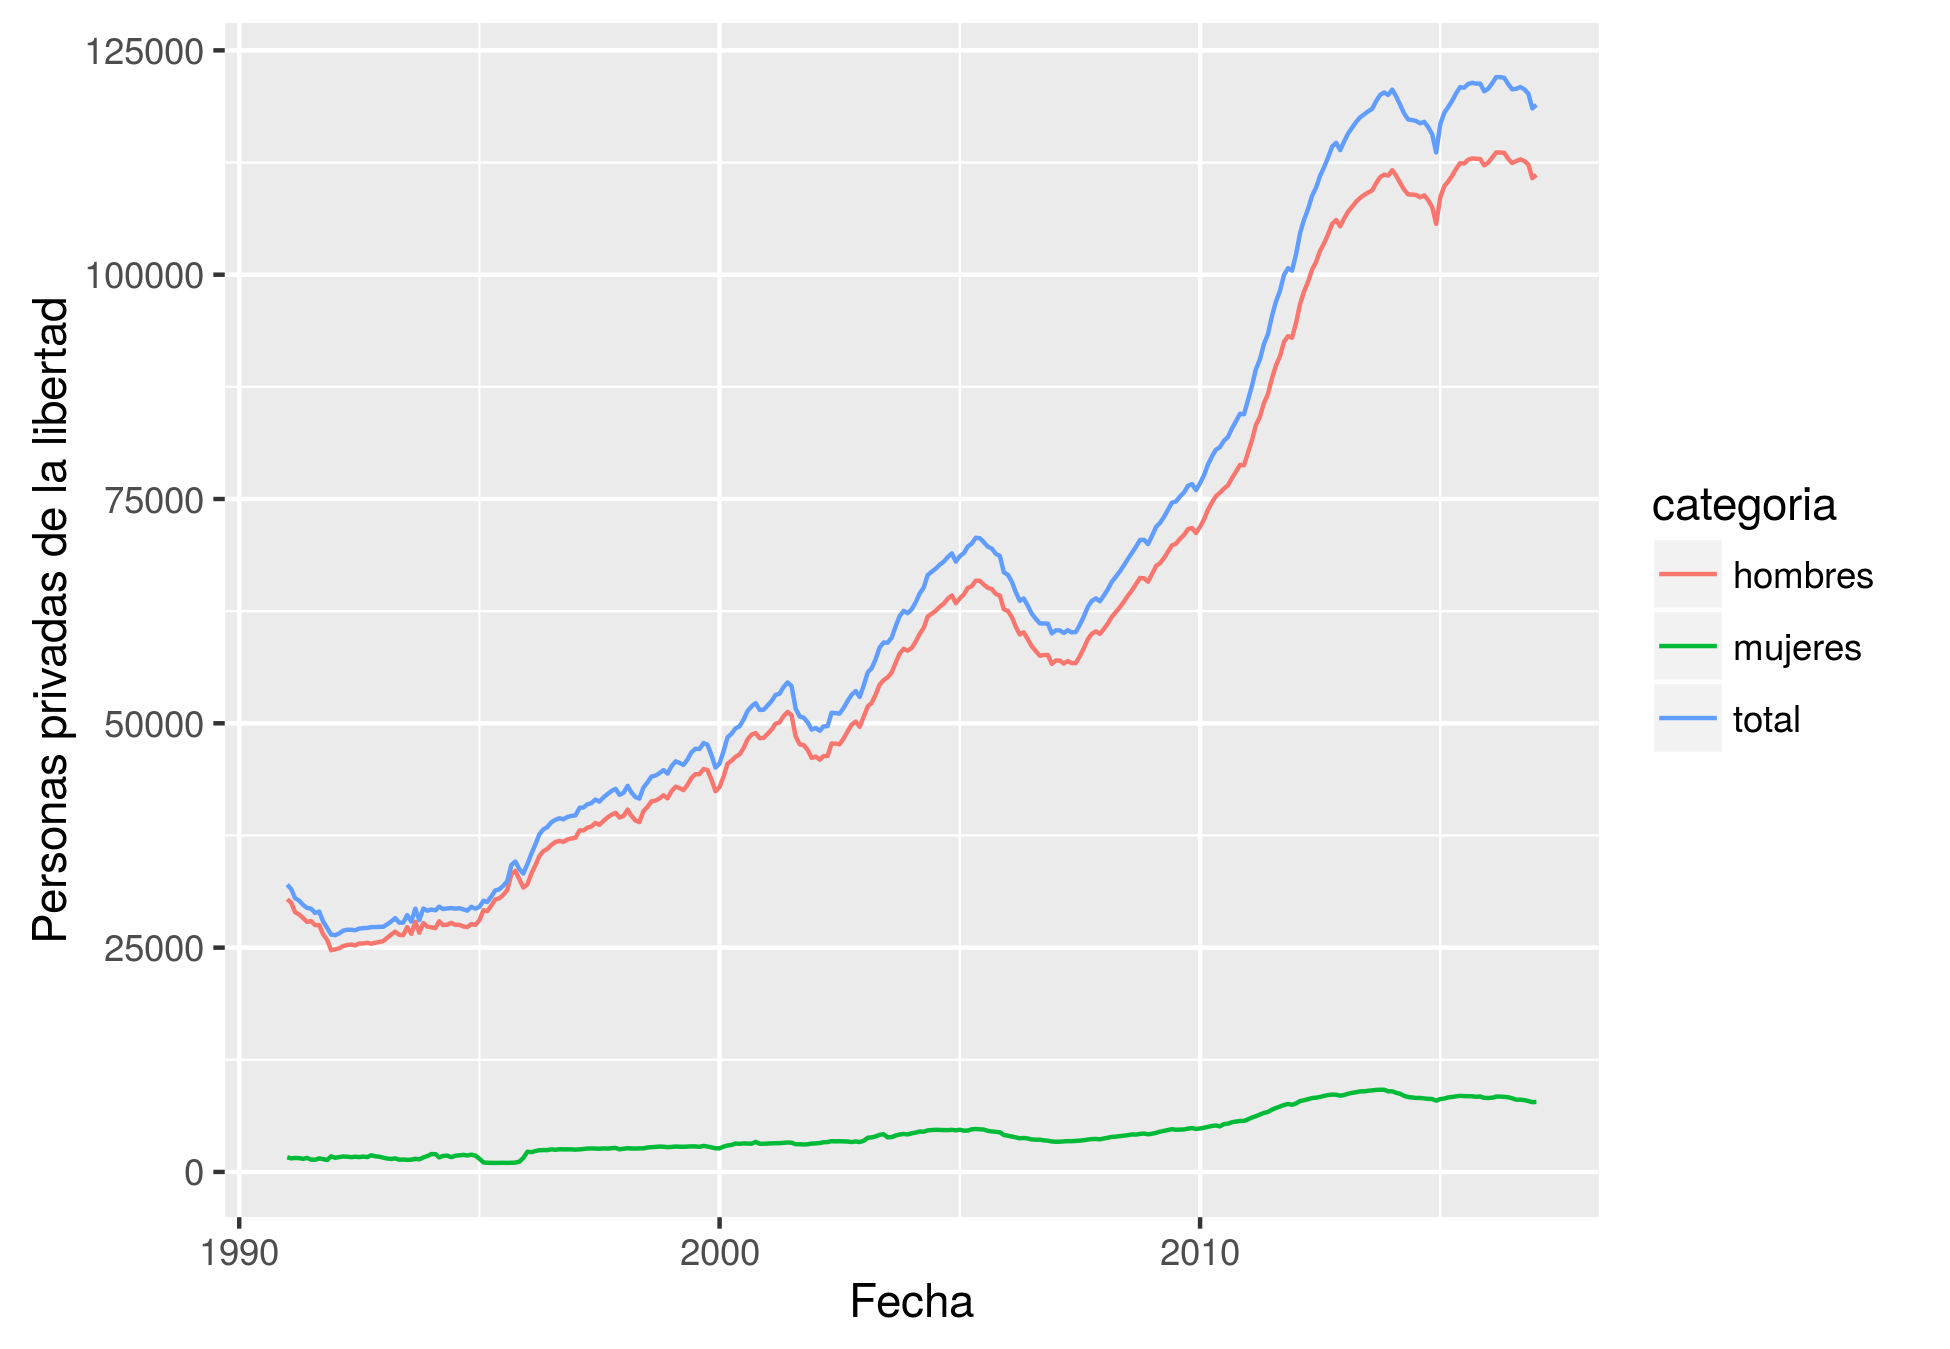
\includegraphics[width=10cm]{genero.png}
	\caption{Poblaci�n privada de la libertad 1991 - 2017} {Fuente: INPEC\\} {Elaboraci�n propia}
	\label{fig:genero}
\end{figure}

El incremento en la poblaci�n carcelaria podr�a tomarse como un efecto del crecimiento de la poblaci�n colombiana. Para validar este supuesto calculamos la tasa de encarcelamiento, que mide la cantidad de personas encarceladas por cada cien mil habitantes. Este indicador pas� de 92 personas por cada cien mil habitantes en enero de 1991 a 242 en enero de 2016. Tal incremento se puede ver tanto en hombres como en mujeres. Ver figura \ref{fig:tasas}. 


\begin{figure}[htb]
	\centering
	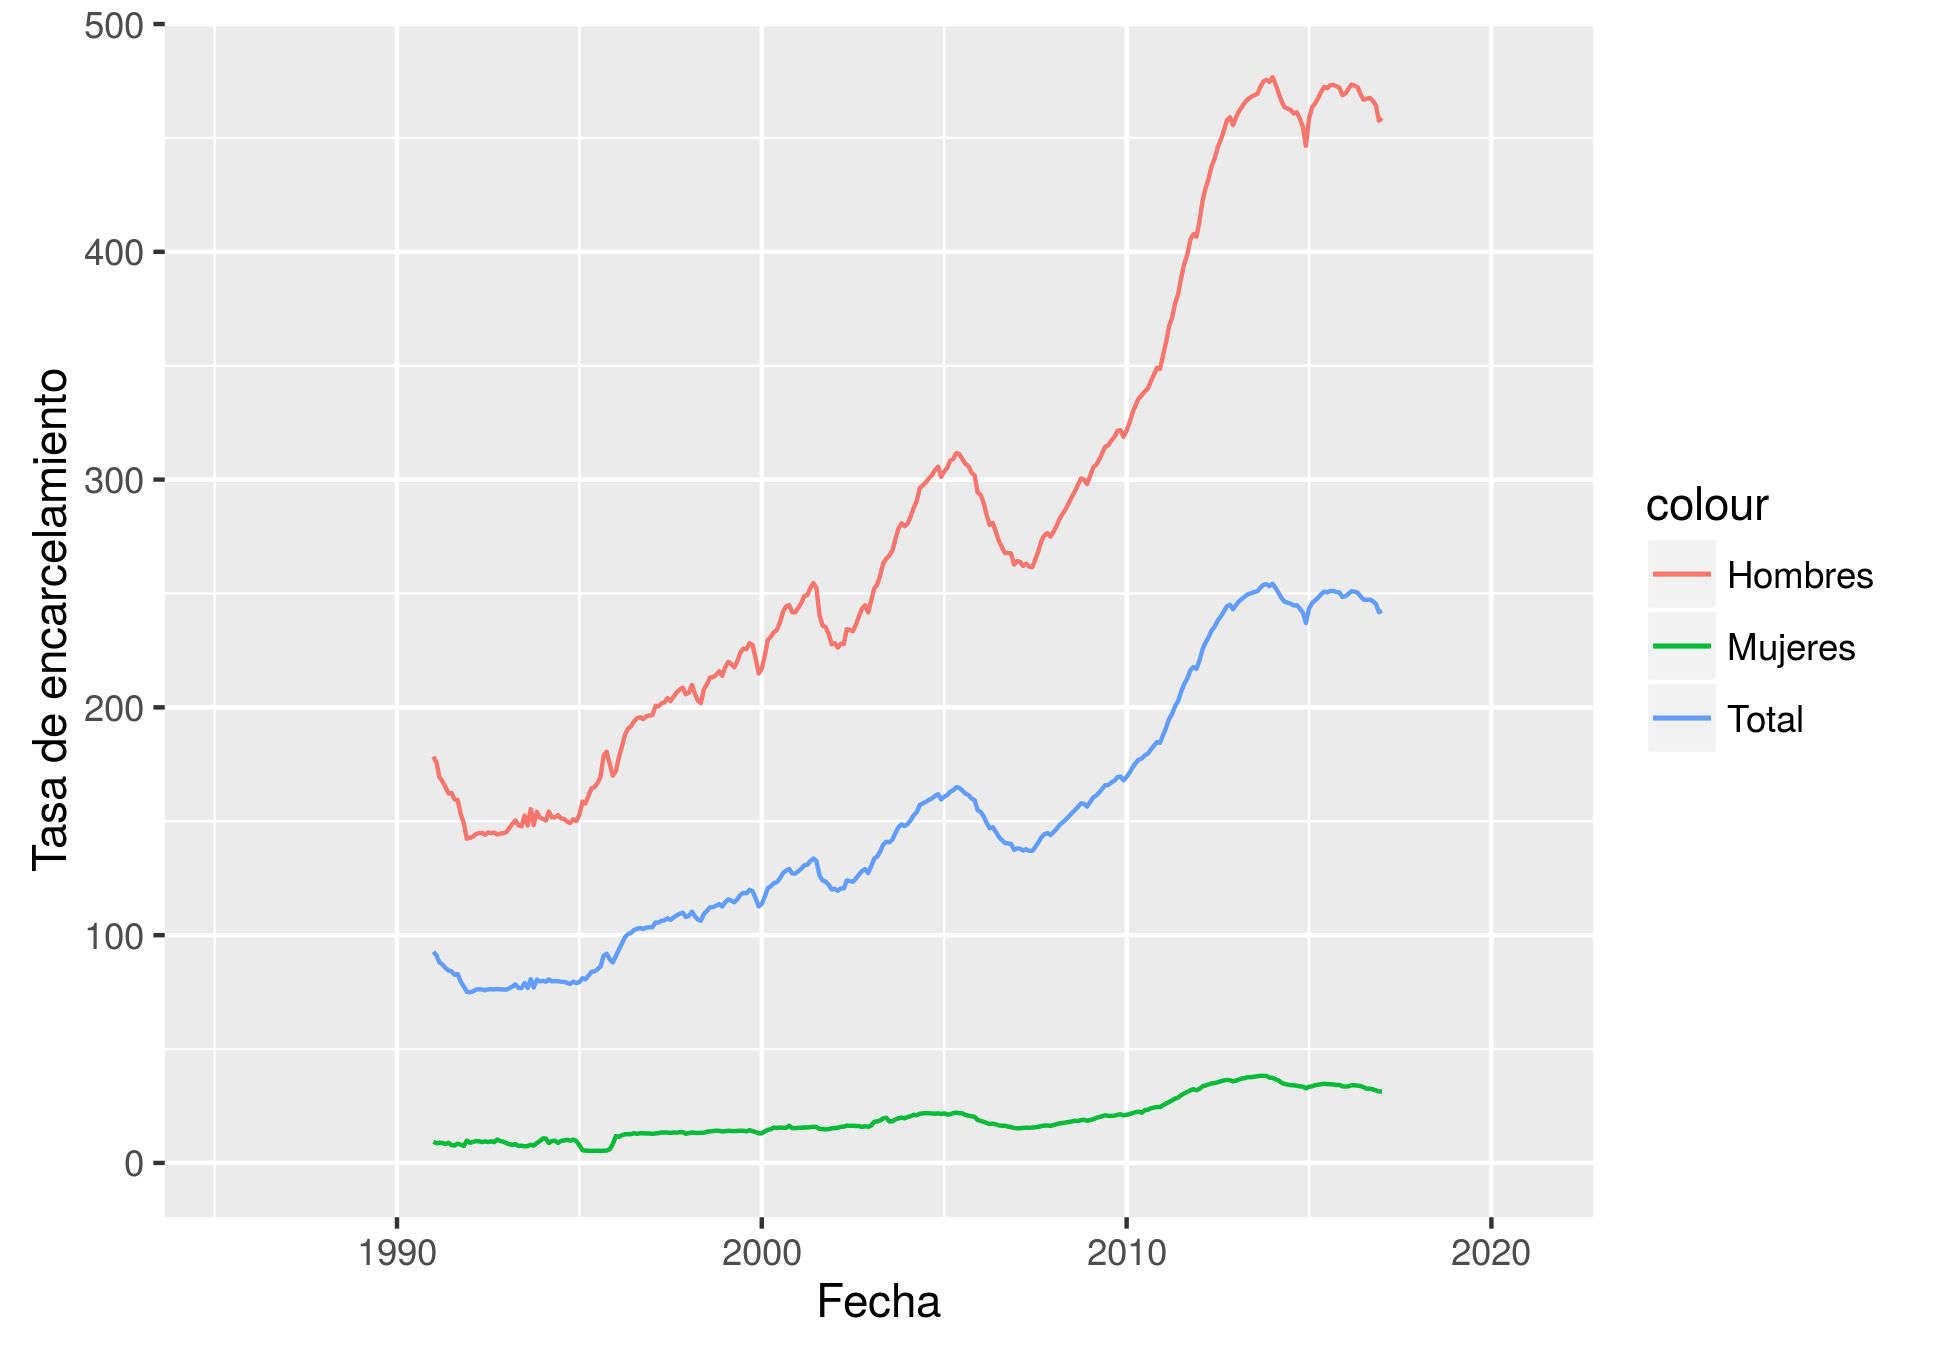
\includegraphics[width=10cm]{tasas}
	\caption{Tasa de encarcelamiento seg�n genero 1991 - 2017\\}{Fuente: INPEC\\} {Elaboraci�n propia}
	\label{fig:tasas}
\end{figure}

La tasa de encarcelamiento es un indicador que var�a seg�n la edad y genero, siendo m�s elevado en los hombres que en las mujeres y m�s algo en los hombres j�venes, que en los hombres mayores (cita pendiente).  Otra posible explicaci�n al cambio en la tasa de encarcelamiento es un cambio en la pir�mide poblacional en el periodo analizado. No obstante, no podemos confirmar o refutar esta hip�tesis pues la serie de tiempo, contenida en los datos de libre acceso no se encuentra desagregada por edad.

\section{El sistema penitenciario en Colombia}

La poblaci�n carcelaria se ve afectada por dos pol�ticas, la pol�tica penitenciaria, que determina las condiciones de privaci�n de la libertad y la pol�tica criminal que determina las causas de encarcelamiento y la duraci�n de las penas. \cite{DepartamentoNacionaldePlaneacion2015}

A la poblaci�n privada de la libertad antes del juicio se le denomina pobaci�n sindicada, y a aquellos que han sido juzgados y se encuentran cumpliendo la sentencia se les denomina poblaci�n condenada. La evoluci�n de la poblaci�n seg�n situaci�n jur�dica se puede observar en la figura \ref{fig:sit_jur}

\begin{figure}[htb]
	\centering
	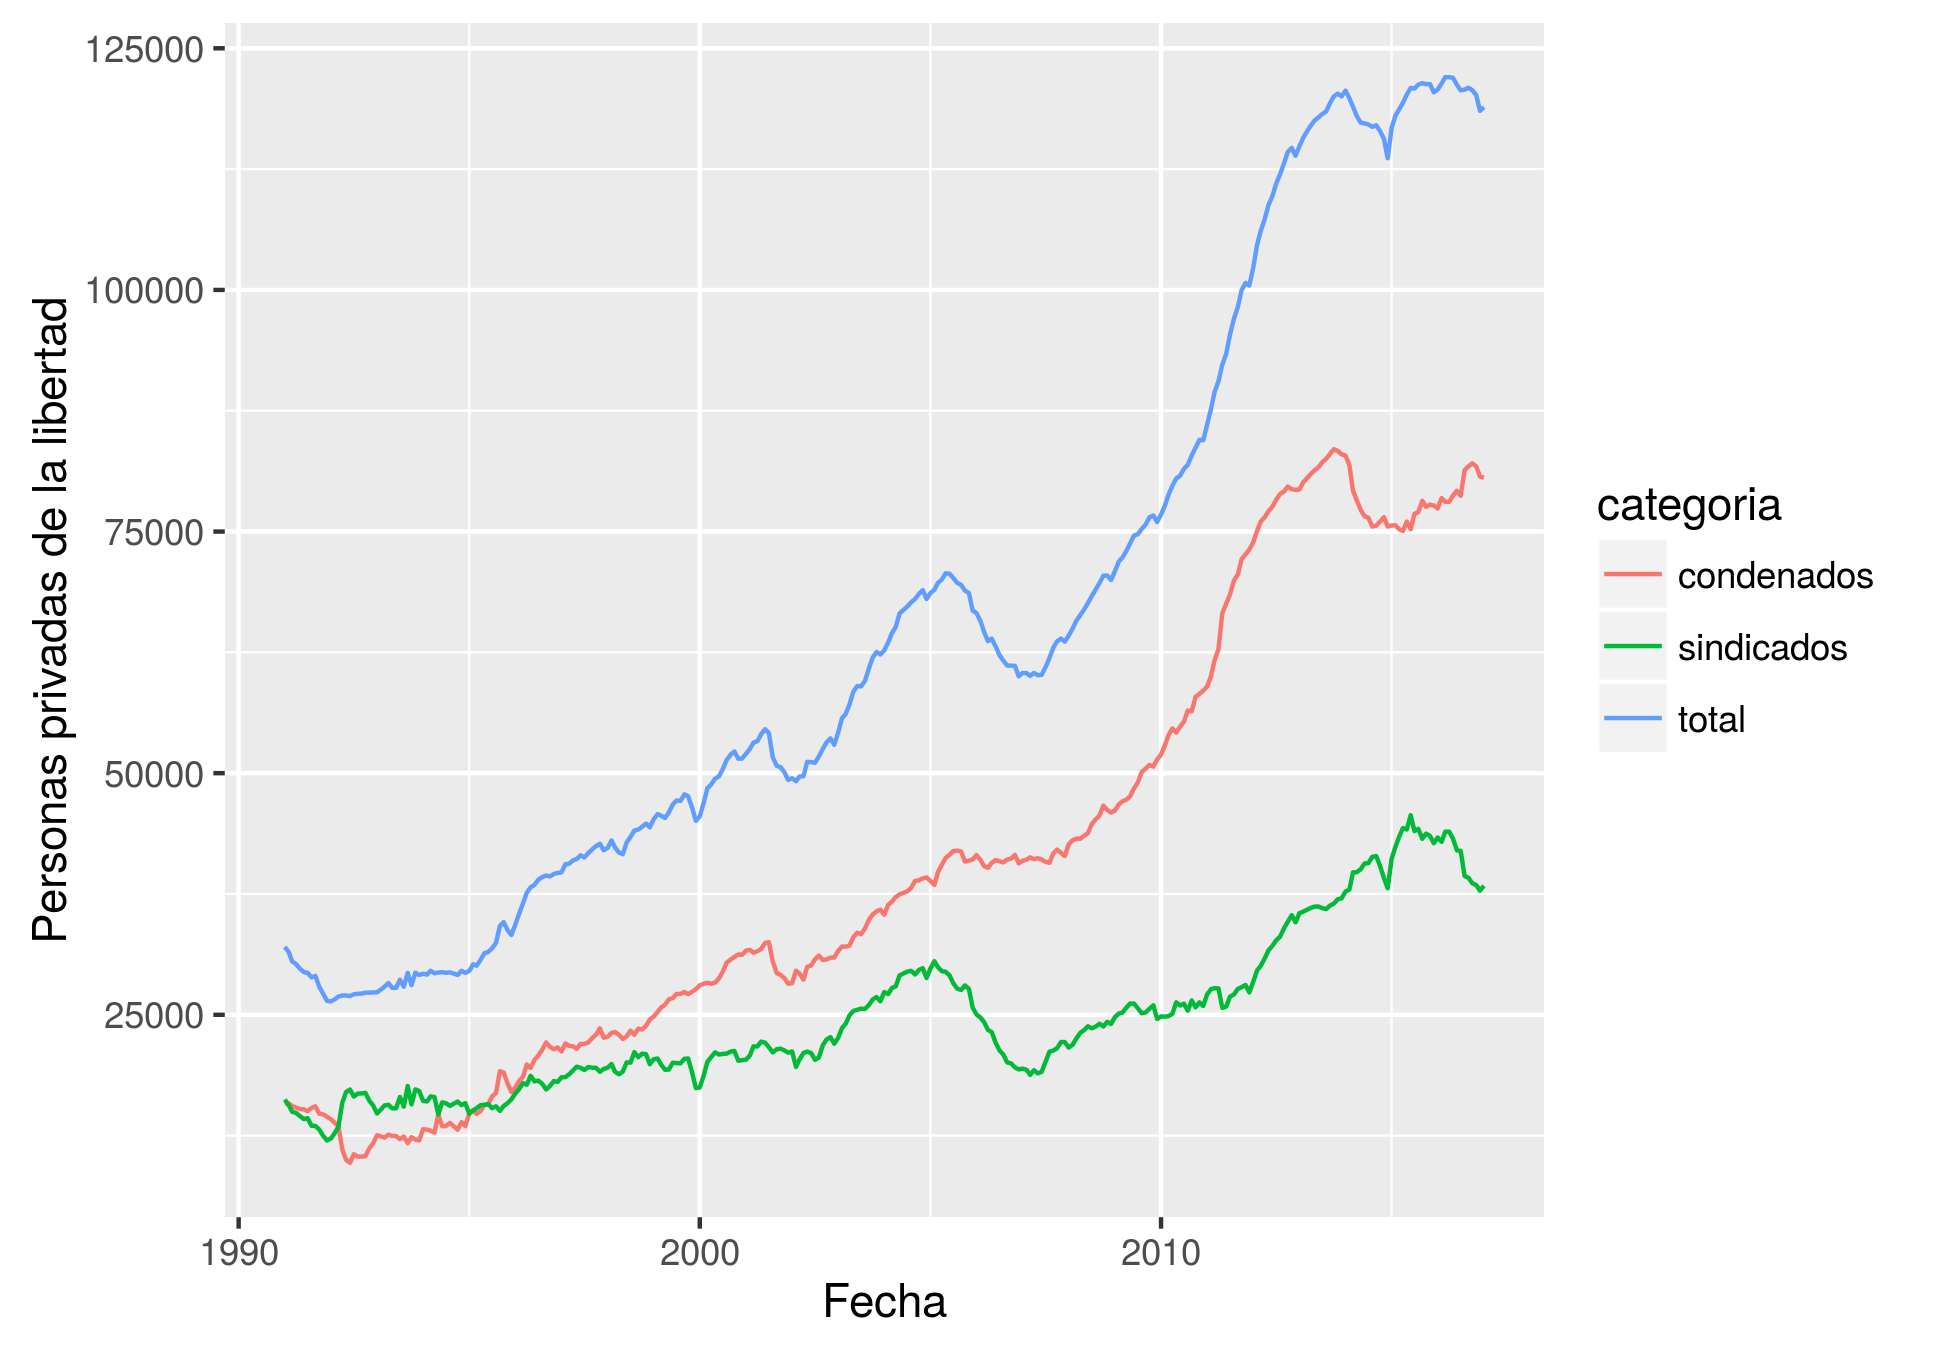
\includegraphics[width=10cm]{sit_jur.png}
	\caption{Poblaci�n carcelaria por situaci�n jur�dica\\} {Fuente: INPEC\\} {Elaboraci�n propia}
	\label{fig:sit_jur}
\end{figure}

\subsection{Identificaci�n del modelo}

Podemos modelar el sistema penitenciario de la siguiente manera:
%
\begin{equation}\label{Sindicados}
	S_t = S_{t-1} + \alpha {N_t} - \gamma S_{t-1}
\end{equation} 
%
\begin{equation}\label{Condenados}
	C_t = C_{t-1} - \omega C_{t-1} + \beta \gamma S_{t-1}
\end{equation} 
%
	$N_t$ = poblaci�n nacional en el periodo t \\
	$S_t$ = poblaci�n de sindicados en el periodo t\\
	$C_t$ = poblaci�n de condenados en el periodo t\\
	$\alpha$ = proporci�n de la poblaci�n libre que ingresa al sistema carcelario \\
	$\gamma$ = proporci�n de sindicados que es juzgada cada periodo \\
	$\beta$ = proporci�n de sindicados que han sido encontrados culpables durante el juicio	\\
	$\omega$ = proporci�n de condenados que cumplen su pena cada\\ periodo.
	
Y esto es un problema interesante porque no tengo las series de tiempo de la transici�n! 
    \chapter{Modelos SARIMA}

La estimaci�n de los modelos se realiza usando el paquete base del software R \cite{RCoreTeam2017}, y el paquete astsa \cite{Stoffer2014}, cuyo uso es discutido en detalle por Shumway \cite{Shumway}. 

En adelante nos referiremos a la funci�n de auctocorrelaci�n como ACF y a la funci�n de autocorrelaci�n parcial como PACF. 

\section{Identificaci�n del modelo}

% Variaci�n poblaci�n total, sindicada y condenada
\begin{figure}[H]
	\centering
	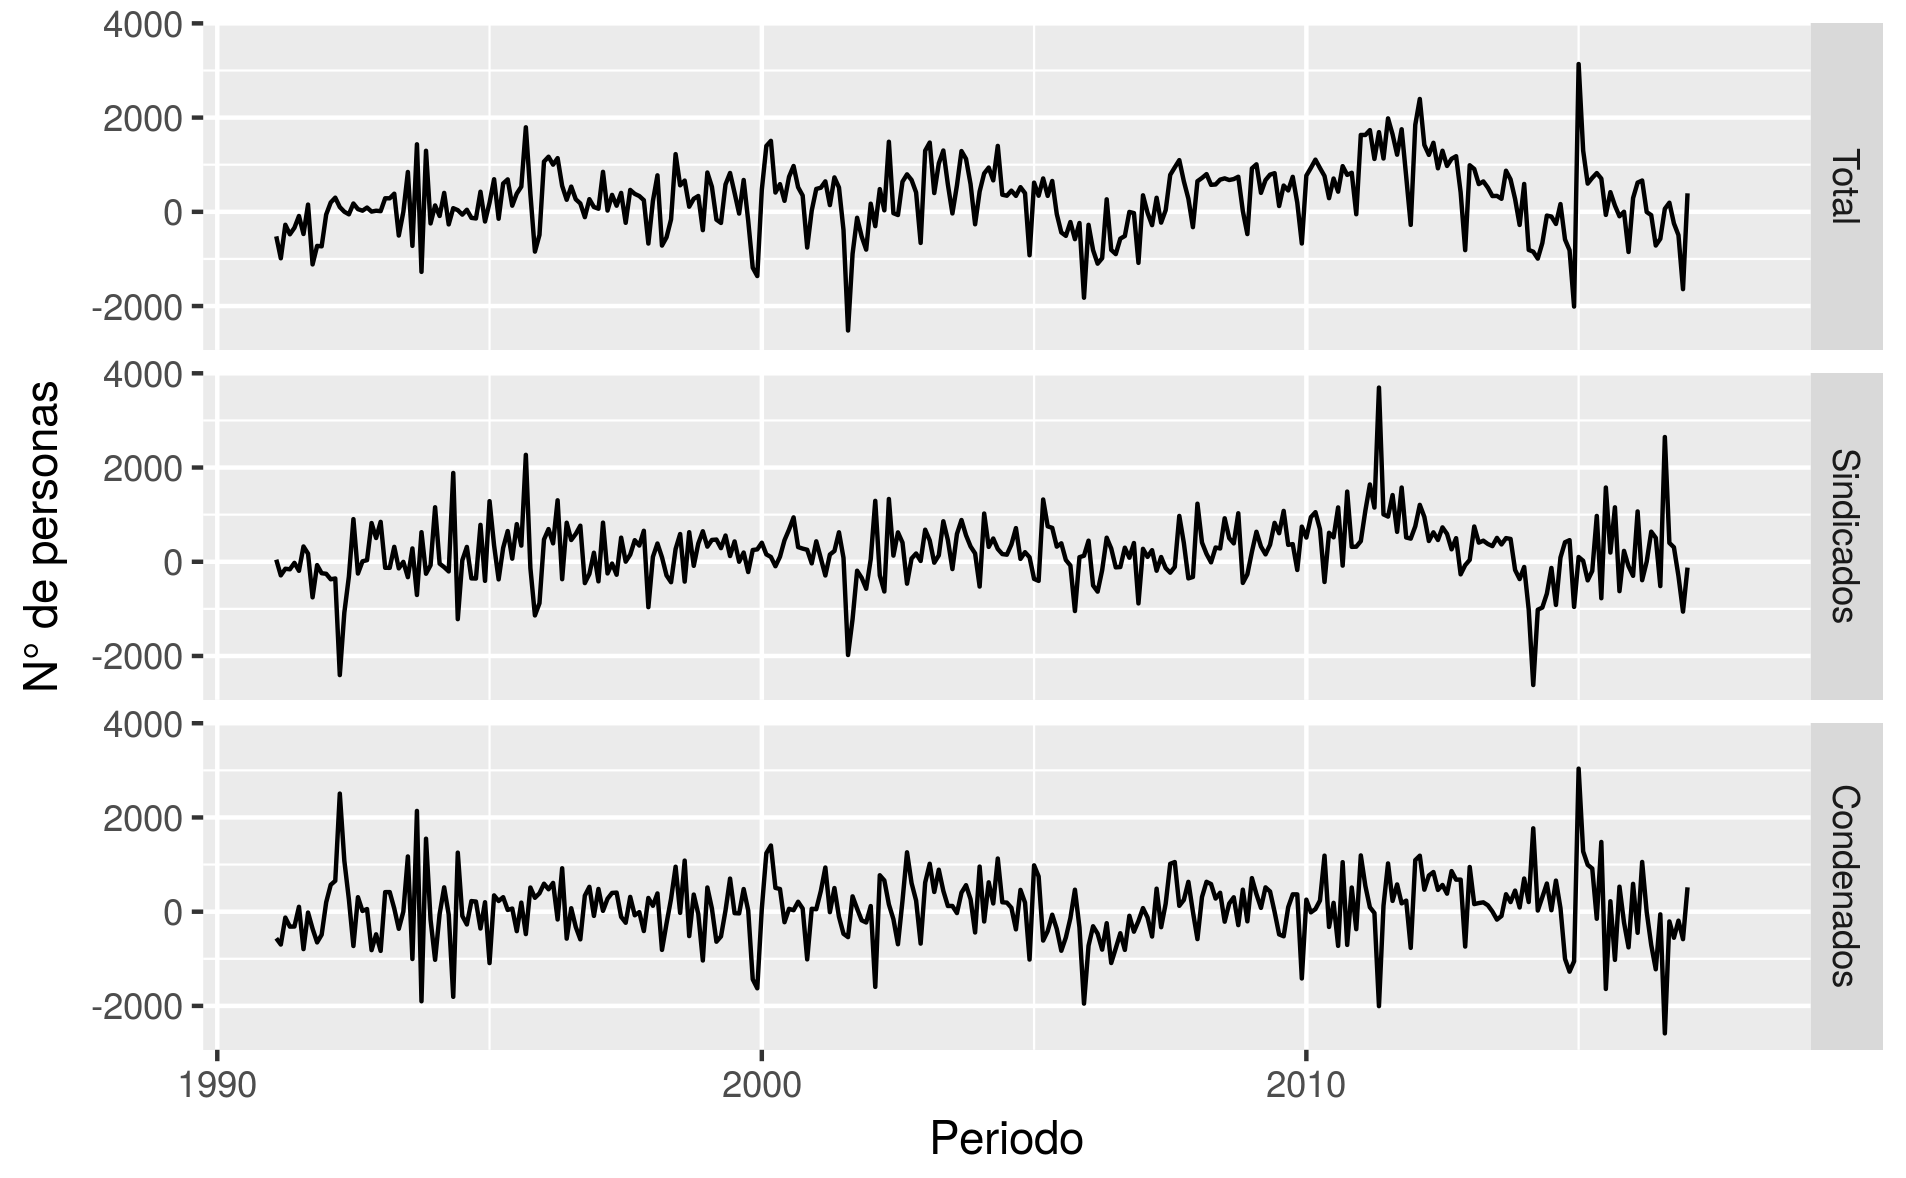
\includegraphics[width=0.7\linewidth]{variacion_intermensual}
	\caption[Variaci�n inter-mensual de poblaci�n carcelaria]{Variaci�n inter-mensual de poblaci�n carcelaria, sindicados y condenados}
	\label{fig:variacion_intermensual}
\end{figure}

Antes de realizar la proyecci�n de una serie de tiempo, es necesario identificar el modelo que explique adecuadamente su comportamiento. 

Aunque conocemos, por la estructura del proceso que genera los datos, que las series de tiempo de poblaci�n sindicada y condenada no son independientes, podemos simplificar la proyecci�n, trat�ndolas como independientes. En este caso, los modelos ARIMA y SARIMA resultan apropiados, pues permiten explicar separadamente cada observaci�n en funci�n del comportamiento hist�rico de la serie.

El cap�tulo anterior suger�a que la poblaci�n carcelaria, tanto sindicada como condenada, tiene una marcada tendencia al alza. En este caso una herramienta �til es mostrar gr�ficamente la variaci�n mes a mes de la poblaci�n. \ref{fig:variacion_intermensual}. Para tener una mejor estrucutura de an�lisis usamos la funci�n "decompose" de R base. 

La serie tiene un componente estacional marcado, con una reducci�n de la poblaci�n carcelaria en diciembre. La variabilidad del componente aleatorio es elevada. La tendencia parece tener cambios estructurales en algunos periodos, por ejemplo reducci�n de la poblaci�n carcelaria entre 2005-2007,  y 2012 - 2015, e incrementos de la poblaci�n de magnitud mayor al promedio entre 2008 y 2012.

La mayor parte de la variaci�n de la poblaci�n total se puede asociar con variaciones en a poblaci�n sindicada \ref{fig:variacion_mensual_sindicados_desc}. La poblaci�n condenada tiene una tendencia con una tendencia m�s estable.  \ref{fig:variacion_mensual_condenados_desc}

% Descomposici�n variaci�n poblaci�n total
\begin{figure}[H]
\centering
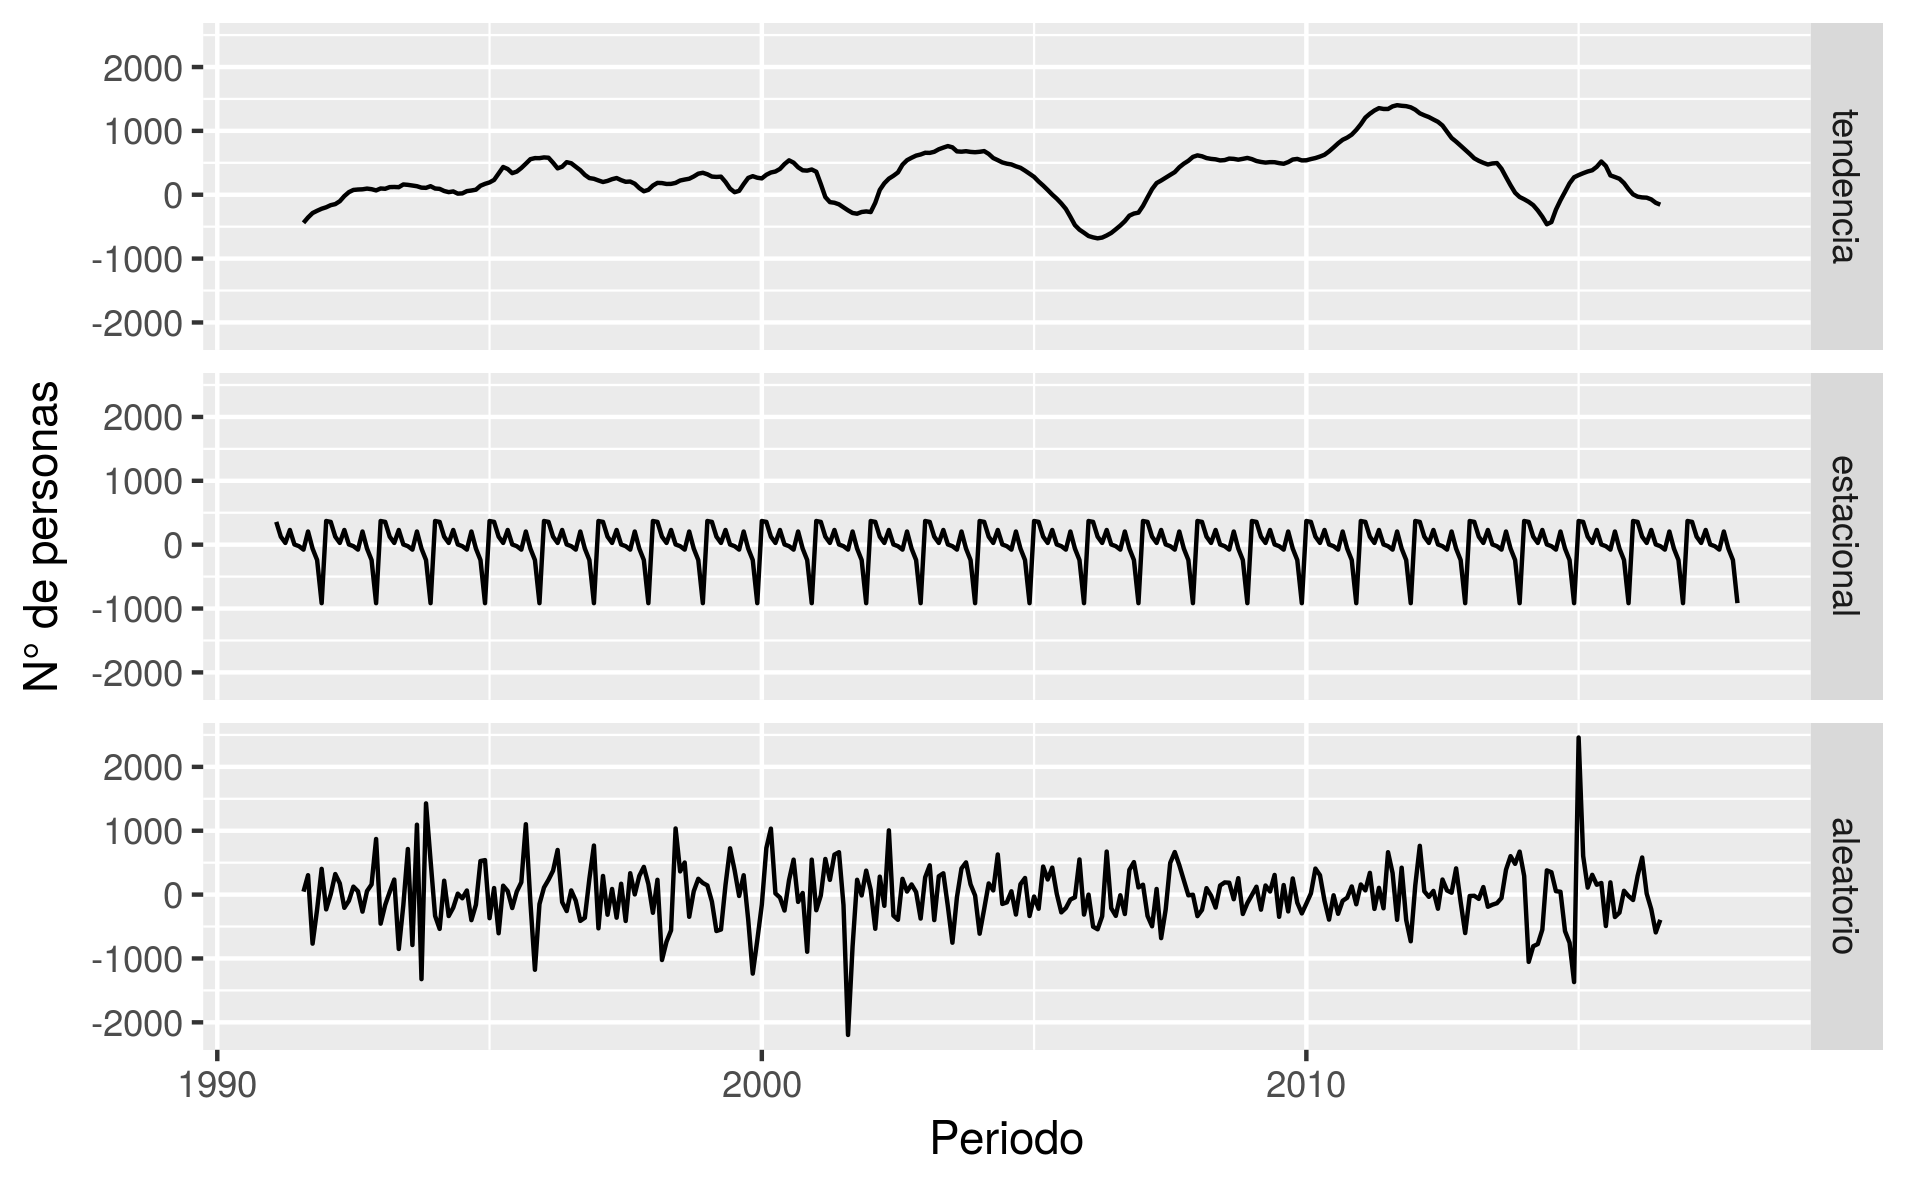
\includegraphics[width=0.7\linewidth]{variacion_mensual_total_desc}
\caption[Descomposici�n de la variaci�n inter-mensual de poblaci�n carcelaria total]{Variaci�n mensual de poblaci�n carcelaria descompuesta por tendencia, estacionalidad y componente aleatorio.}
\label{fig:variacion_mensual_total_desc}
\end{figure}

% Descomposici�n variaci�n poblaci�n sindicada
\begin{figure}[H]
	\centering
	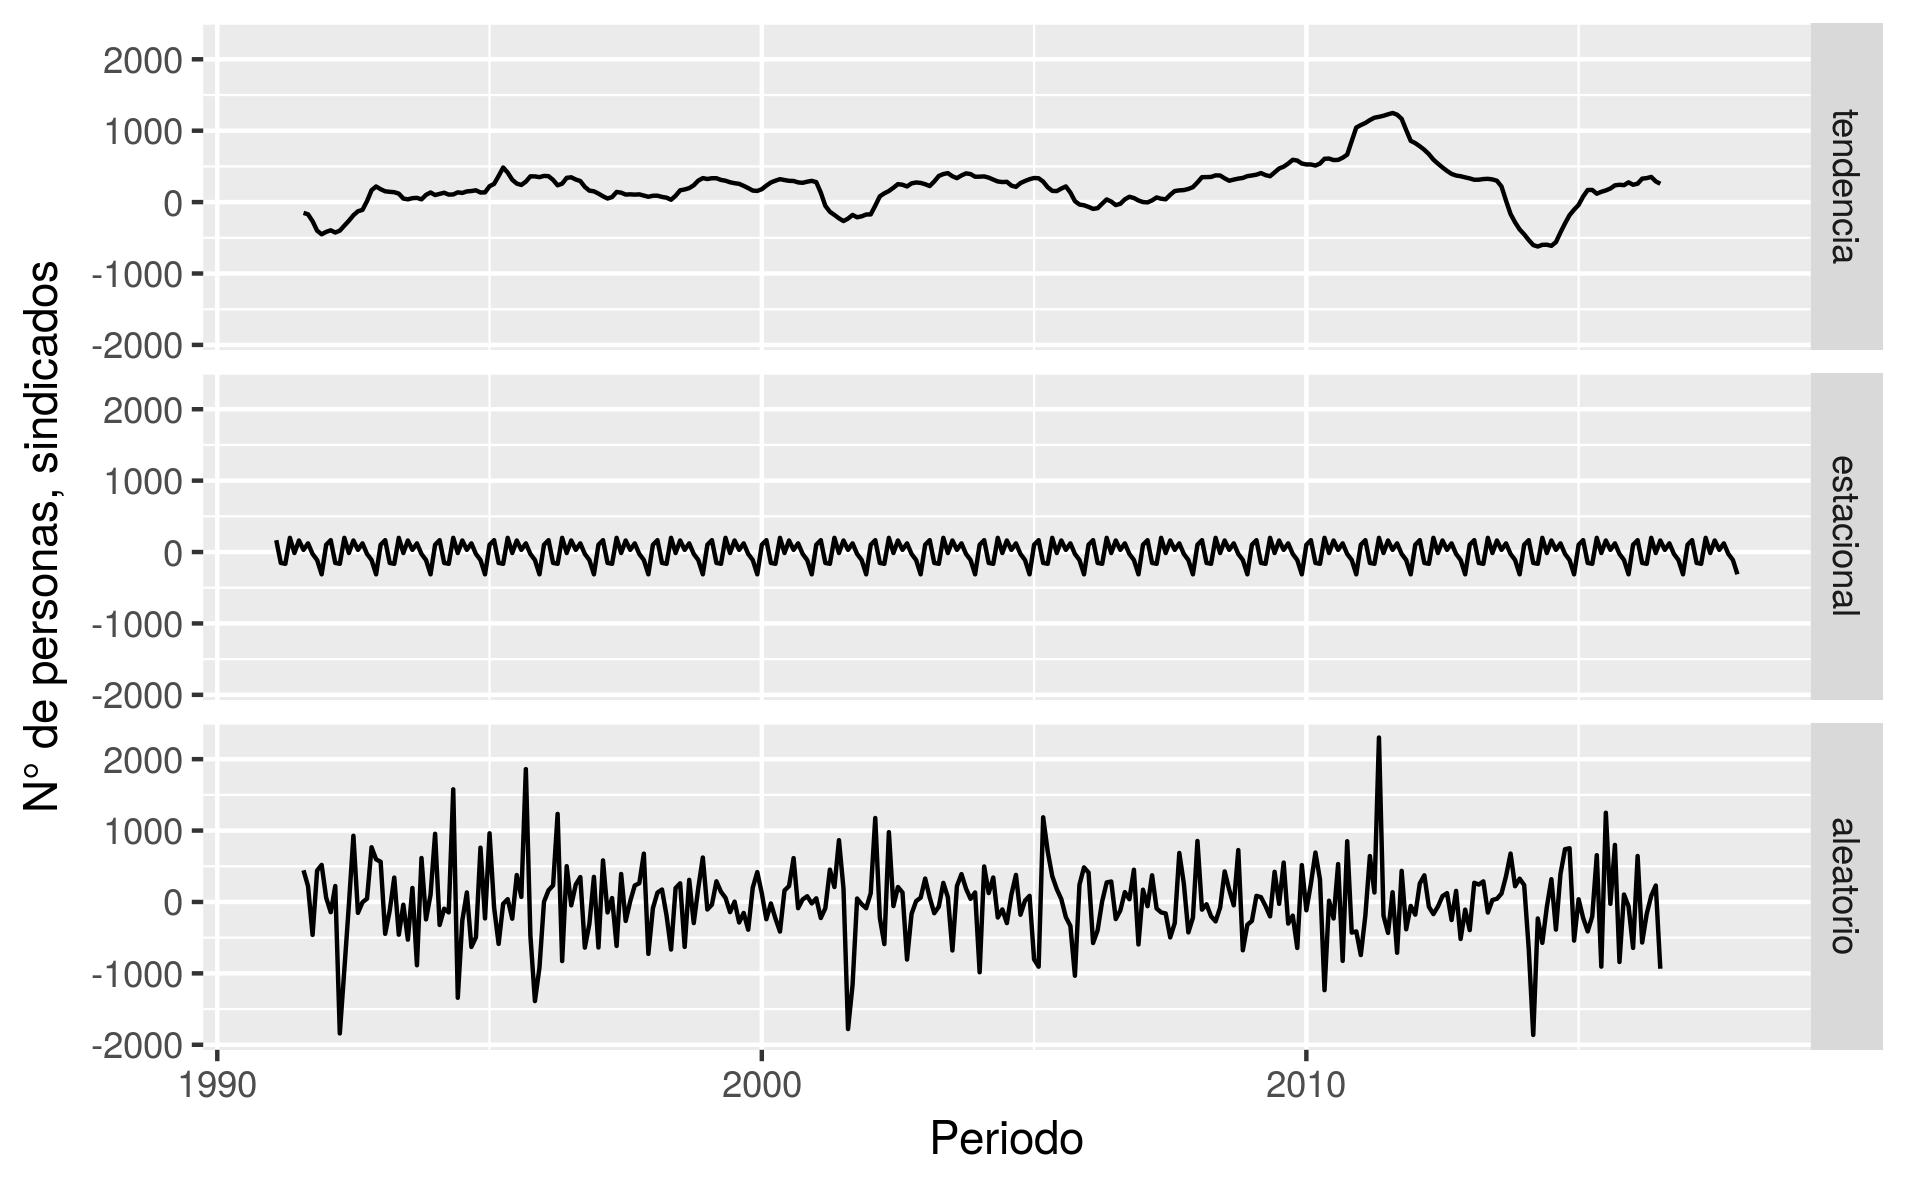
\includegraphics[width=0.7\linewidth]{variacion_mensual_sindicados_desc}
	\caption[Descomposici�n de la variaci�n inter-mensual de poblaci�n carcelaria total]{Variaci�n mensual de poblaci�n carcelaria sindicada,  descompuesta por tendencia, estacionalidad y componente aleatorio.}
	\label{fig:variacion_mensual_sindicados_desc}
\end{figure}

% Descomposici�n variaci�n poblaci�n condenada
\begin{figure}[H]
	\centering
	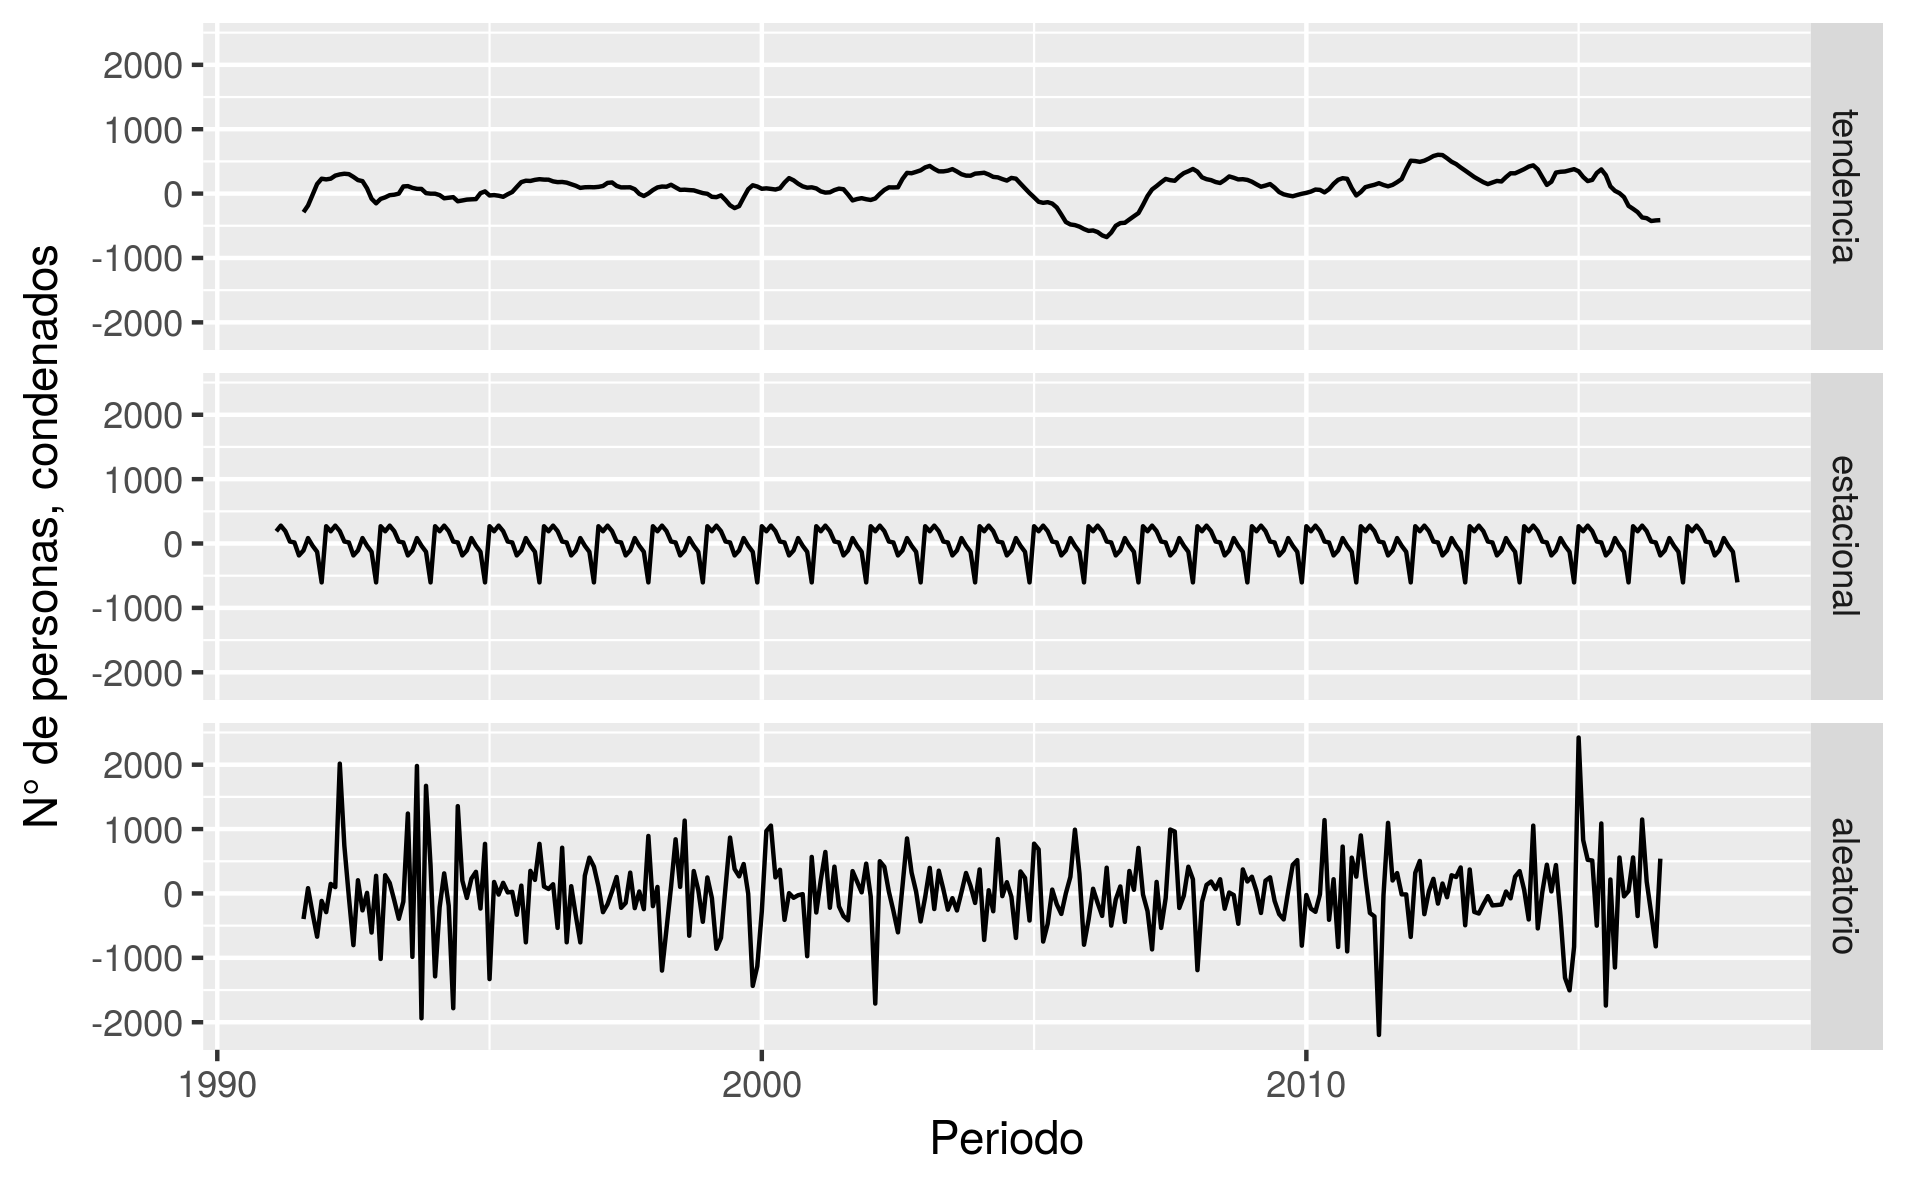
\includegraphics[width=0.7\linewidth]{variacion_mensual_condenados_desc}
	\caption[Descomposici�n de la variaci�n inter-mensual de poblaci�n carcelaria total]{Variaci�n mensual de poblaci�n carcelaria condenada,  descompuesta por tendencia, estacionalidad y componente aleatorio.}
	\label{fig:variacion_mensual_condenados_desc}
\end{figure}


Se trabaja sobre la diferencia de cada serie de tiempo con lag 1 y lag 12, al observar que la serie tiene un crecimiento sostenido entre 1991 y 2017, sugiriendo un proceso estocastico integrado. Sobre cada serie (poblaci�n total, poblaci�n sindicadda y poblaci�n condenada)  se realiza la funci�n de autocorrelaci�n y autocorrelaci�n parcial y se presenta en la figura \ref{fig:ACF_variacion_mensual}. Estas funciones son usadas como herramienta de diagn�stico, para intuir modelos adecuados en cada serie.

Con base en la tabla \ref{ARMA_ACF} se realiza una revisi�n del comportamiento de las series de poblaci�n carcelaria, poblaci�n sindicada y poblaci�n condenada.

% Pendiente traducir este fragmento
\begin{table}[H]
	\centering
	\caption{Comportamiento de la ACF y PACF en modelos ARMA(p,q) \cite{Shumway}}
	\label{ARMA_ACF}
	\begin{tabular}{lllll}
		\multicolumn{1}{|l|}{}              & \multicolumn{1}{c|}{\textbf{AR(p)}}       & \multicolumn{1}{c|}{\textbf{MA(q)}}       & \multicolumn{1}{c|}{\textbf{ARMA(p,q)}} &  \\ \cline{1-4}
		\multicolumn{1}{|l|}{\textbf{ACF}}  & \multicolumn{1}{l|}{Tails off}            & \multicolumn{1}{l|}{Cuts off after lag q} & \multicolumn{1}{l|}{Tails off}          &  \\ \cline{1-4}
		\multicolumn{1}{|l|}{\textbf{PACF}} & \multicolumn{1}{l|}{Cuts off after lag p} & \multicolumn{1}{l|}{Tails off}            & \multicolumn{1}{l|}{Tails off}          &  \\ \cline{1-4}
	\end{tabular}
\end{table}


\begin{figure}[H]
	\centering
	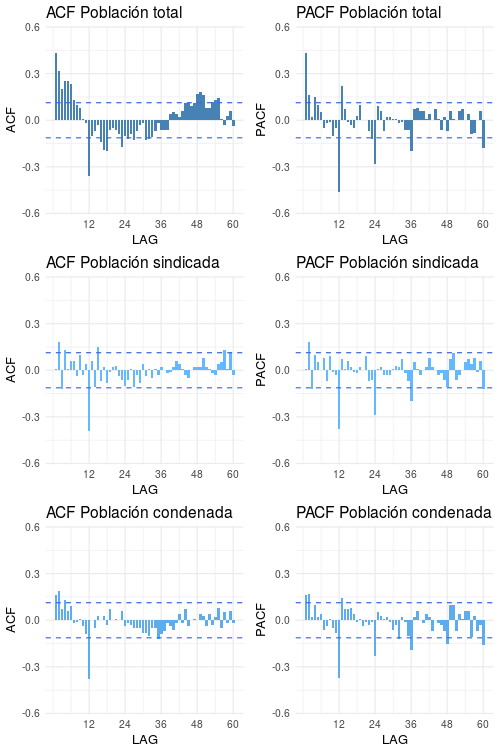
\includegraphics[width=0.7\linewidth]{ACF_var_pob}
	\caption[Autocorrelaci�n parcial de la variaci�n inter-mensual]{Autocorrelaci�n parcial de la variaci�n inter-mensual de la poblaci�n}
	\label{fig:ACF_variacion_mensual}
\end{figure}

\subsection{Poblaci�n total}

La tabla \ref{ARMA_ACF} presenta una gu�a para la interpretaci�n de la ACF y la PACF. En la \ref{fig:ACF_variacion_mensual} podemos observar que tanto la ACF como la PACF decaen lentamente. La APCF decae progresivamente en los meses 12, 24, 36, mientra que la ACF se corta en el lag 24, lo que sugiere que el proceso es un promedio m�vil de orden 1 en el componente estacional.

En este caso una primera estimaci�n se realiza para la proyecci�n de la poblaci�n total como SARIMA(1,1,1,0,0,1)


\subsection{Poblaci�n sindicada}

En la \ref{fig:ACF_variacion_mensual} podemos observar que la ACF decae lentamente, mientras la PACF cae por debajo del error luego del lag 1. La APCF decae progresivamente en los meses 12, 24, 36, mientra que la ACF se corta en el lag 12, lo que sugiere que el proceso es un promedio m�vil de orden 1 en el componente estacional.

En este caso una primera estimaci�n se realiza para la proyecci�n de la poblaci�n sindicada como SARIMA(1,1,1,0,0,1)

\subsection{Poblaci�n condenada}

El comportamiento de la ACF y la PACF es similar al de la poblaci�n sindicada, sugiriendo el mismo modelo: SARIMA(1,1,1,0,0,1).

\section{Estimaci�n de par�mtetros}
El proceso de estimaci�n se realizar� para cada serie por separado, luego se validar� la efectividad de incluir m�s par�metros, usando como criterio de comparaci�n el BIC. A modo informativo se usa la funci�n auto.arima del paquete forecast, para seleccionar el modelo con menor AIC. \cite{Hyndman2017}  
 \cite{Hyndman2008} 
 
\subsection{Poblaci�n total}

\subsection{Poblaci�n sindicada}

\subsection{Poblaci�n condenada}


\section{Proyecci�n}

\subsection{Poblaci�n total}

\subsection{Poblaci�n sindicada}

\subsection{Poblaci�n condenada}

\section{Conclusiones}

Al usar un ARIMA
    \chapter{PROYECCIONES CON MODELOS ESTADO ESPACIO}

\section{Marco te�rico}

\section{Identificaci�n del modelo}

\section{Simulaci�n Monte-Carlo}

\section{Estimaci�n de par�metros}

\section{Proyecciones 2017 - 2020}

\section{Conclusiones}
%\appendix
%    \chapter{Gr�ficas adicionales}

\begin{figure}[htb]
 \centering
 
\includegraphics[width=10cm]{small_escudo_color}
 \caption{Escudo oficial de la UN a color dise�ado por el Maestro Francisco Duarte.}
 \label{fig:escudo_color}
\end{figure}


\begin{table}
\centering
\caption{Unidades de \TeX.}
\begin{tabular}{l|l}\hline
\verb"mm" & mil�metro $\approx$ 1/25 pulgada \\
\verb"cm" & cent�metro = 10 mm \\
\verb"in" & pulgada $\approx$ 25 mm \\
\verb"pt" & punto $\approx$ 1/72 pulgada $\approx$ 1/3 mm \\
\verb"em" & aprox. el ancho de una m en el tipo actual \\
\verb"ex" & aprox. la altura de una x en el tipo actual \\\hline
\end{tabular}
\end{table}

\begin{table}
\centering\renewcommand{\arraystretch}{2}
\caption{Tama�os de los tipos de fuentes \LaTeX.}
 \begin{tabular}{ll|ll}\hline
{\tiny\verb"\tiny"} & {\tiny letra diminuta}
& {\large\verb"\large"} & {\large letra grande} \\
{\scriptsize\verb"\scriptsize"} & {\scriptsize letra muy peque�a}
& {\Large\verb"\Large"} & {\Large letra mayor} \\
{\footnotesize\verb"\footnotesize"} & {\footnotesize letra bastante peque�a}
& {\LARGE\verb"\LARGE"} & {\LARGE muy grande} \\
{\small\verb"\small"} & {\small letra peque�a}
& {\huge\verb"\huge"} & {\huge enorme} \\
\verb"\normalsize" & letra normal
& {\Huge\verb"\Huge"} & {\Huge la mayor} \\\hline
 \end{tabular}
\end{table}





\backmatter
    \conclusion{conclusiones}
    \futurework{trabajofuturo}
%    \glossary{glosario}
%\nocite{*}
    \bibliography{references}
    %\printindex
\end{document}
